%
% A Real Chapter
\chapter{Background}\label{chap:background}
In this chapter, a brief background on walking preliminaries, related works to \ac{CoM} height variation and humanoid robotics at \ac{IHMC} is given.
% Modeling of Walking
\section{Walking Preliminaries}
Different models have different limitations and advantages. Identifying the differences is important to develop an insight on how height variation can influence the system dynamics of a walking robot.
% lip
\subsection{Simple Walking Models}
In simple walking models, a devision can be made in the following three categories:
\begin{itemize}
	\item Point-mass with point-foot
	\item Point-mass with finite-sized support polygon
	\item Mass with intertia with finite-sized support polygon
\end{itemize}
In the point-mass with point-foot model, the only \ac{GRF} that can be generated intersects with both the point-mass and the point-foot. The addition of a finite-sized support polygon allows the \ac{GRF} to intersect with anywhere on the support polygon, so more \ac{GRF} directions are possible. The inclusion of angular momentum around the \ac{CoM} in the model takes away the constraint of the \ac{GRF} to go through the \ac{CoM}. An example of the model with inertia and a finite-sized support polygon is the flywheel model. In \figref{fig:flywheel}, the flywheel model with prismatic leg joint is shown. The combined effects of the leg force $\fleg$, the anke torque $\tauankle$ and the torque around the \ac{CoM} $\taucom$ on the mass $m$ with inertia $\mathbf{I}$ determine the direction and magnitude of the resulting \ac{GRF} $\fgr$. The \ac{GRF} determines together with the external forces, in this example only the gravity vector $\vect{g}$, the linear acceleration $\ddcxyz$ of the \ac{CoM}.
\begin{figure}[h]
\centering
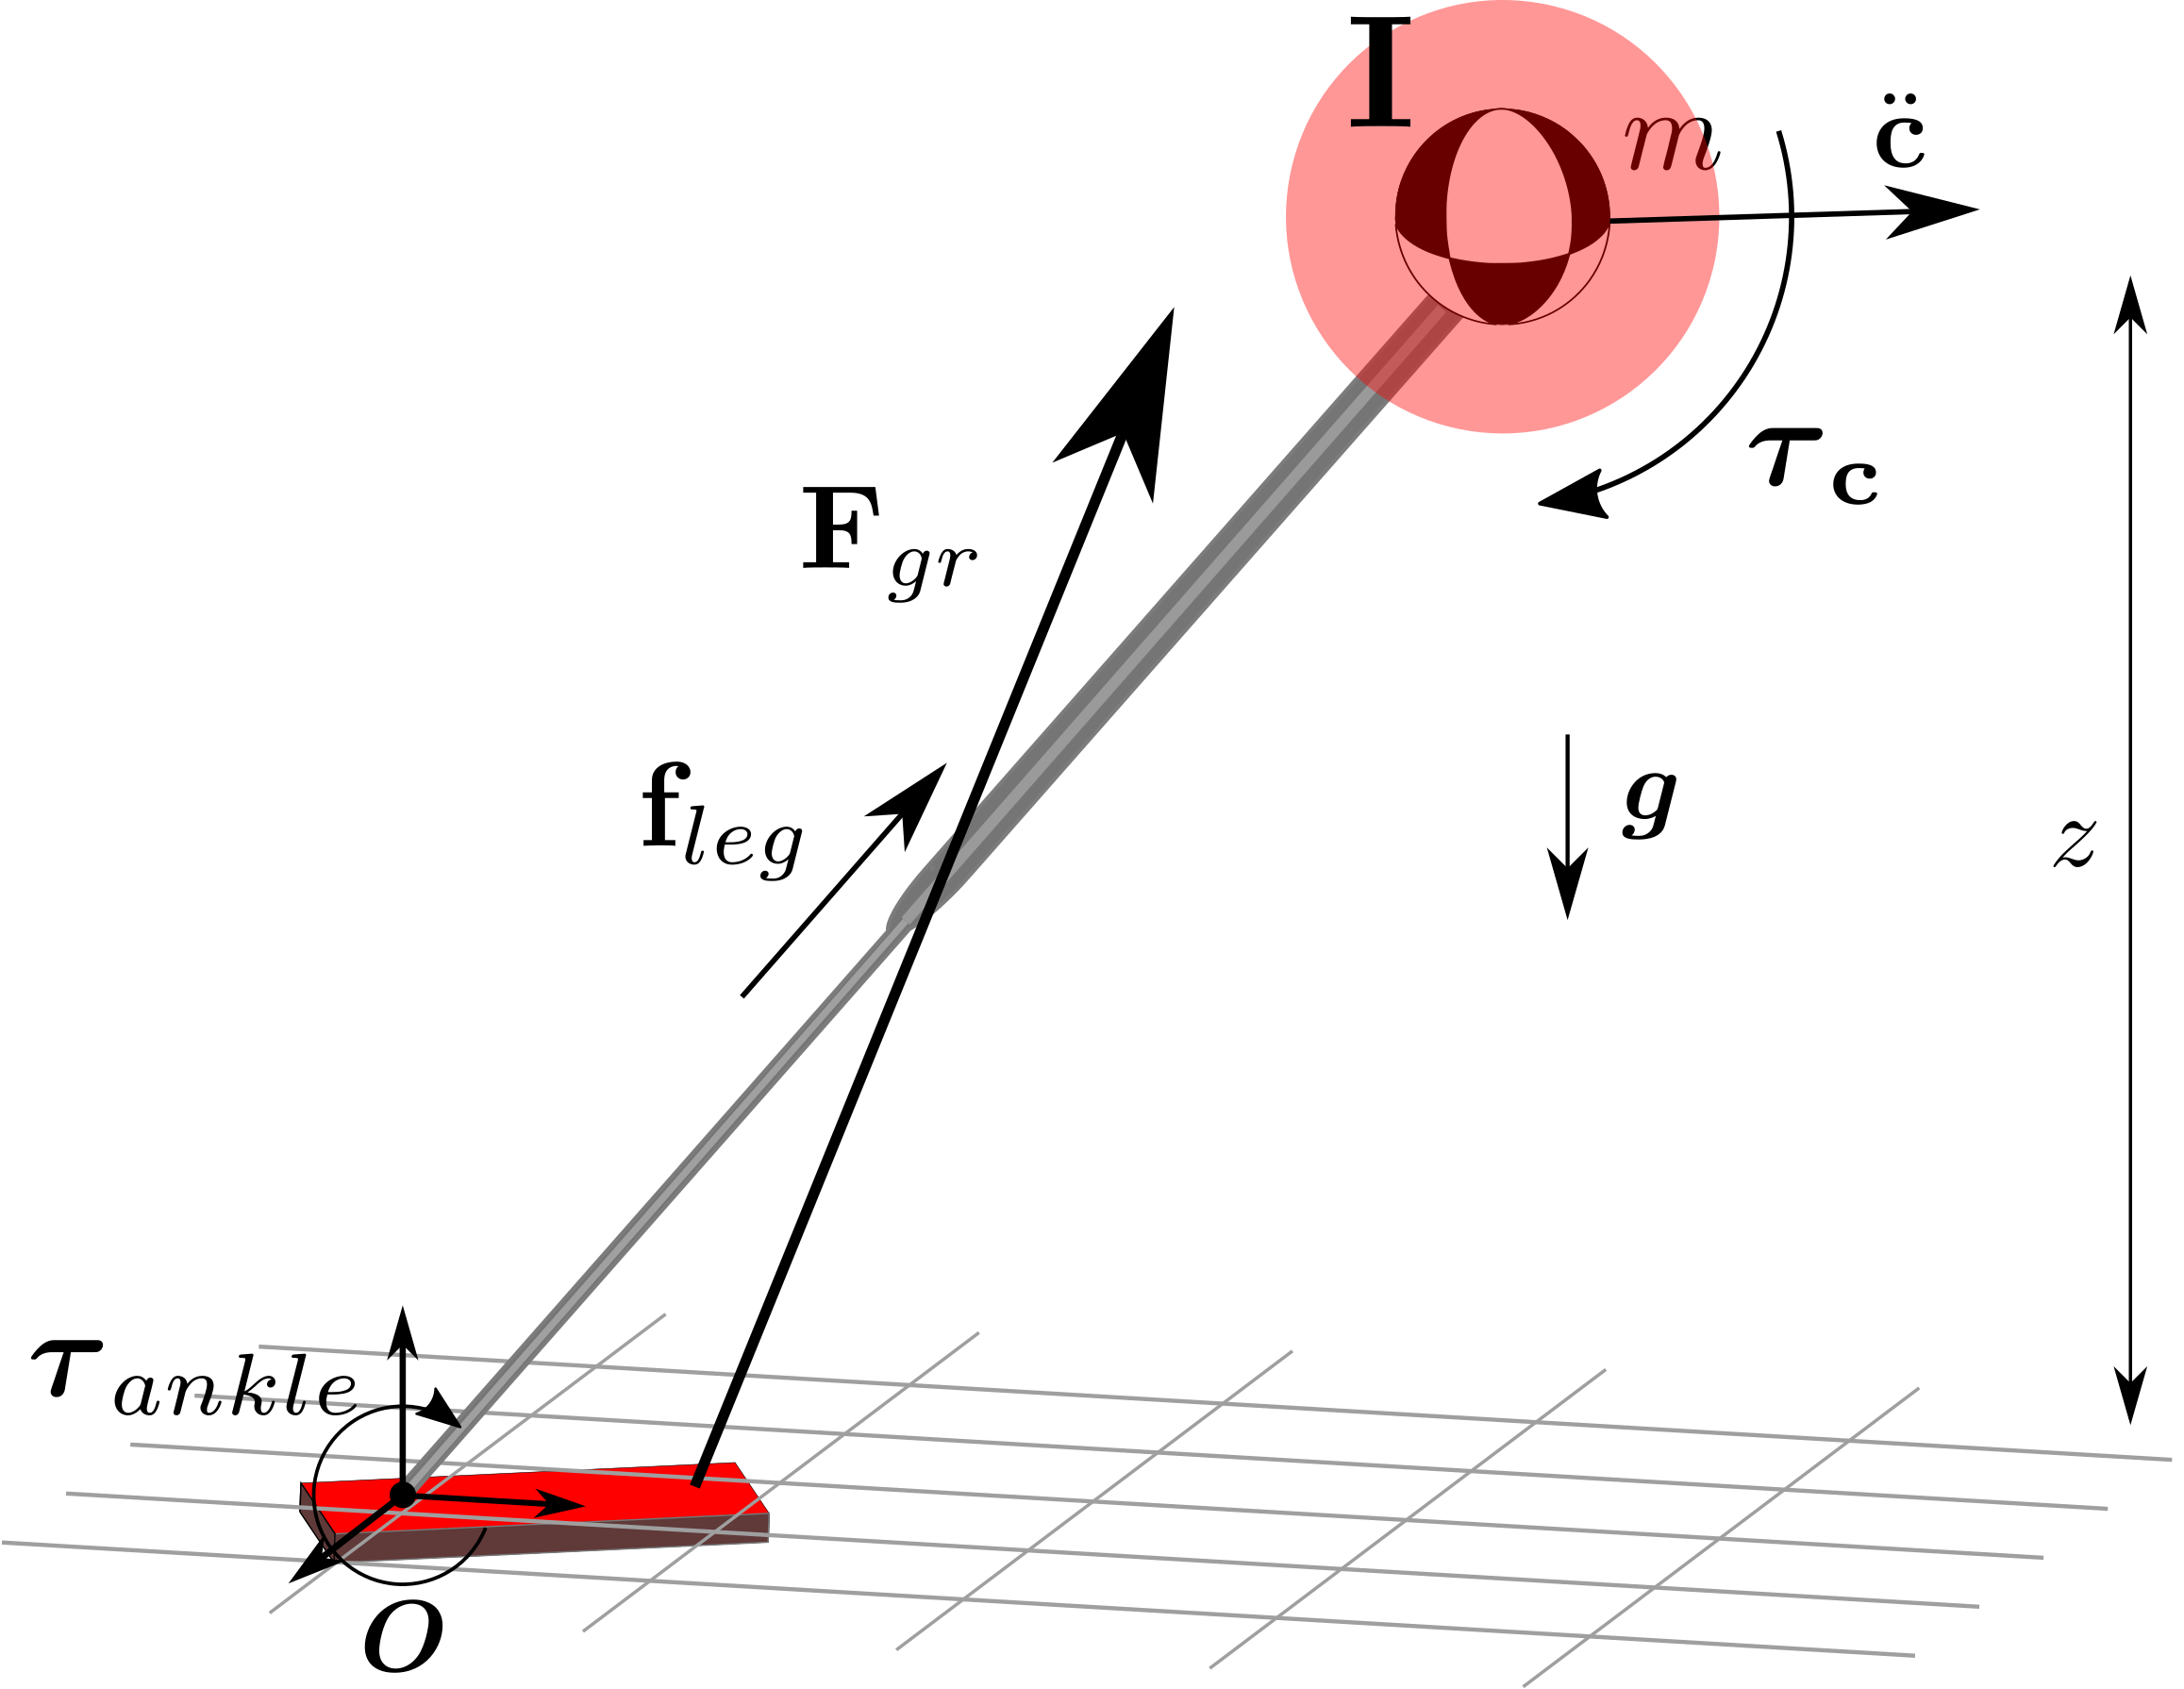
\includegraphics[width=0.5\textwidth]{STYLESTUFF/FlywheelModel.png}
\caption{The flywheel model with finit-sized support polygon.}
\label{fig:flywheel}
\end{figure}

% Ground Reference Points
\subsection{Ground Reference Points}\label{sec:grp}
A common approach for quantifying the dynamics of a walker, either a human or a robot, is the use of ground reference points. Most ground reference points are a function of the state of the robot and the \ac{GRF}.

% ZMP
\paragraph{The zero moment point} is the point on the ground where the resulting \ac{GRF} does not produce any moment in the horizontal plane \cite{sardain2004forces}. By definition, this is also the point where the part of the \ac{GRF} does not cause angular momentum around the \ac{CoM} intersects with the ground surface. The \ac{ZMP} initially was introduced in \cite{vukobratovic1969contribution}. The \ac{ZMP} formulation reads as:
\begin{align}
    x_{zmp}&=x-\frac{\fgrx}{\fgrz}z-\frac{\tau_y}{\fgrz}\\
    y_{zmp}&=y-\frac{\fgrz}{\fgrz}z+\frac{\tau_x}{\fgrz},
\end{align}
where $[\fgrx,\fgry,\fgrz]$ are the components of $\fgr$, $[x,y,z]$ are the components of the \ac{CoM} vector $\cxyz$ and $[\tau_x,-\tau_y]$ are the components of $\taucom$. In \figref{fig:3dlipfoot} the definition of the \ac{ZMP} is visualized in the case of $\inert=0$. 

% CoP
\paragraph{The center of pressure} coincides during walking over flat ground with the \ac{ZMP} \cite{vukobratovic2004zero}.The two points however are not equal in more complex environments. The \ac{CoP} is restricted to be located in the support polygon, while the \ac{ZMP} is restricted to lie on the ground plane  \cite{sardain2004forces}. Traditionally, the \ac{CoP} is a measured quantity from a force pressure plate under the foot.

% CMP
\paragraph{The centroidal moment pivot} includes, unlike the \ac{ZMP} and \ac{CoP}, angular momentum around the \ac{CoM}  \cite{popovic2005ground}. This is defined as the point where a line passing through the \ac{CoM}, parallel to the ground reaction force intersects with the ground surface. The \ac{CMP} is defined as
\begin{align}
    x_{cmp}&=x-\frac{\fgrx}{\fgrz}z\\
    y_{cmp}&=y-\frac{\fgrx}{\fgrz}z.
\end{align}
In \figref{fig:3dlipfootinertia} the difference between the \ac{ZMP} and \ac{CMP} is graphically explained. 

\begin{figure}[h]
\centering
\begin{subfigure}{0.49\textwidth}
\centering
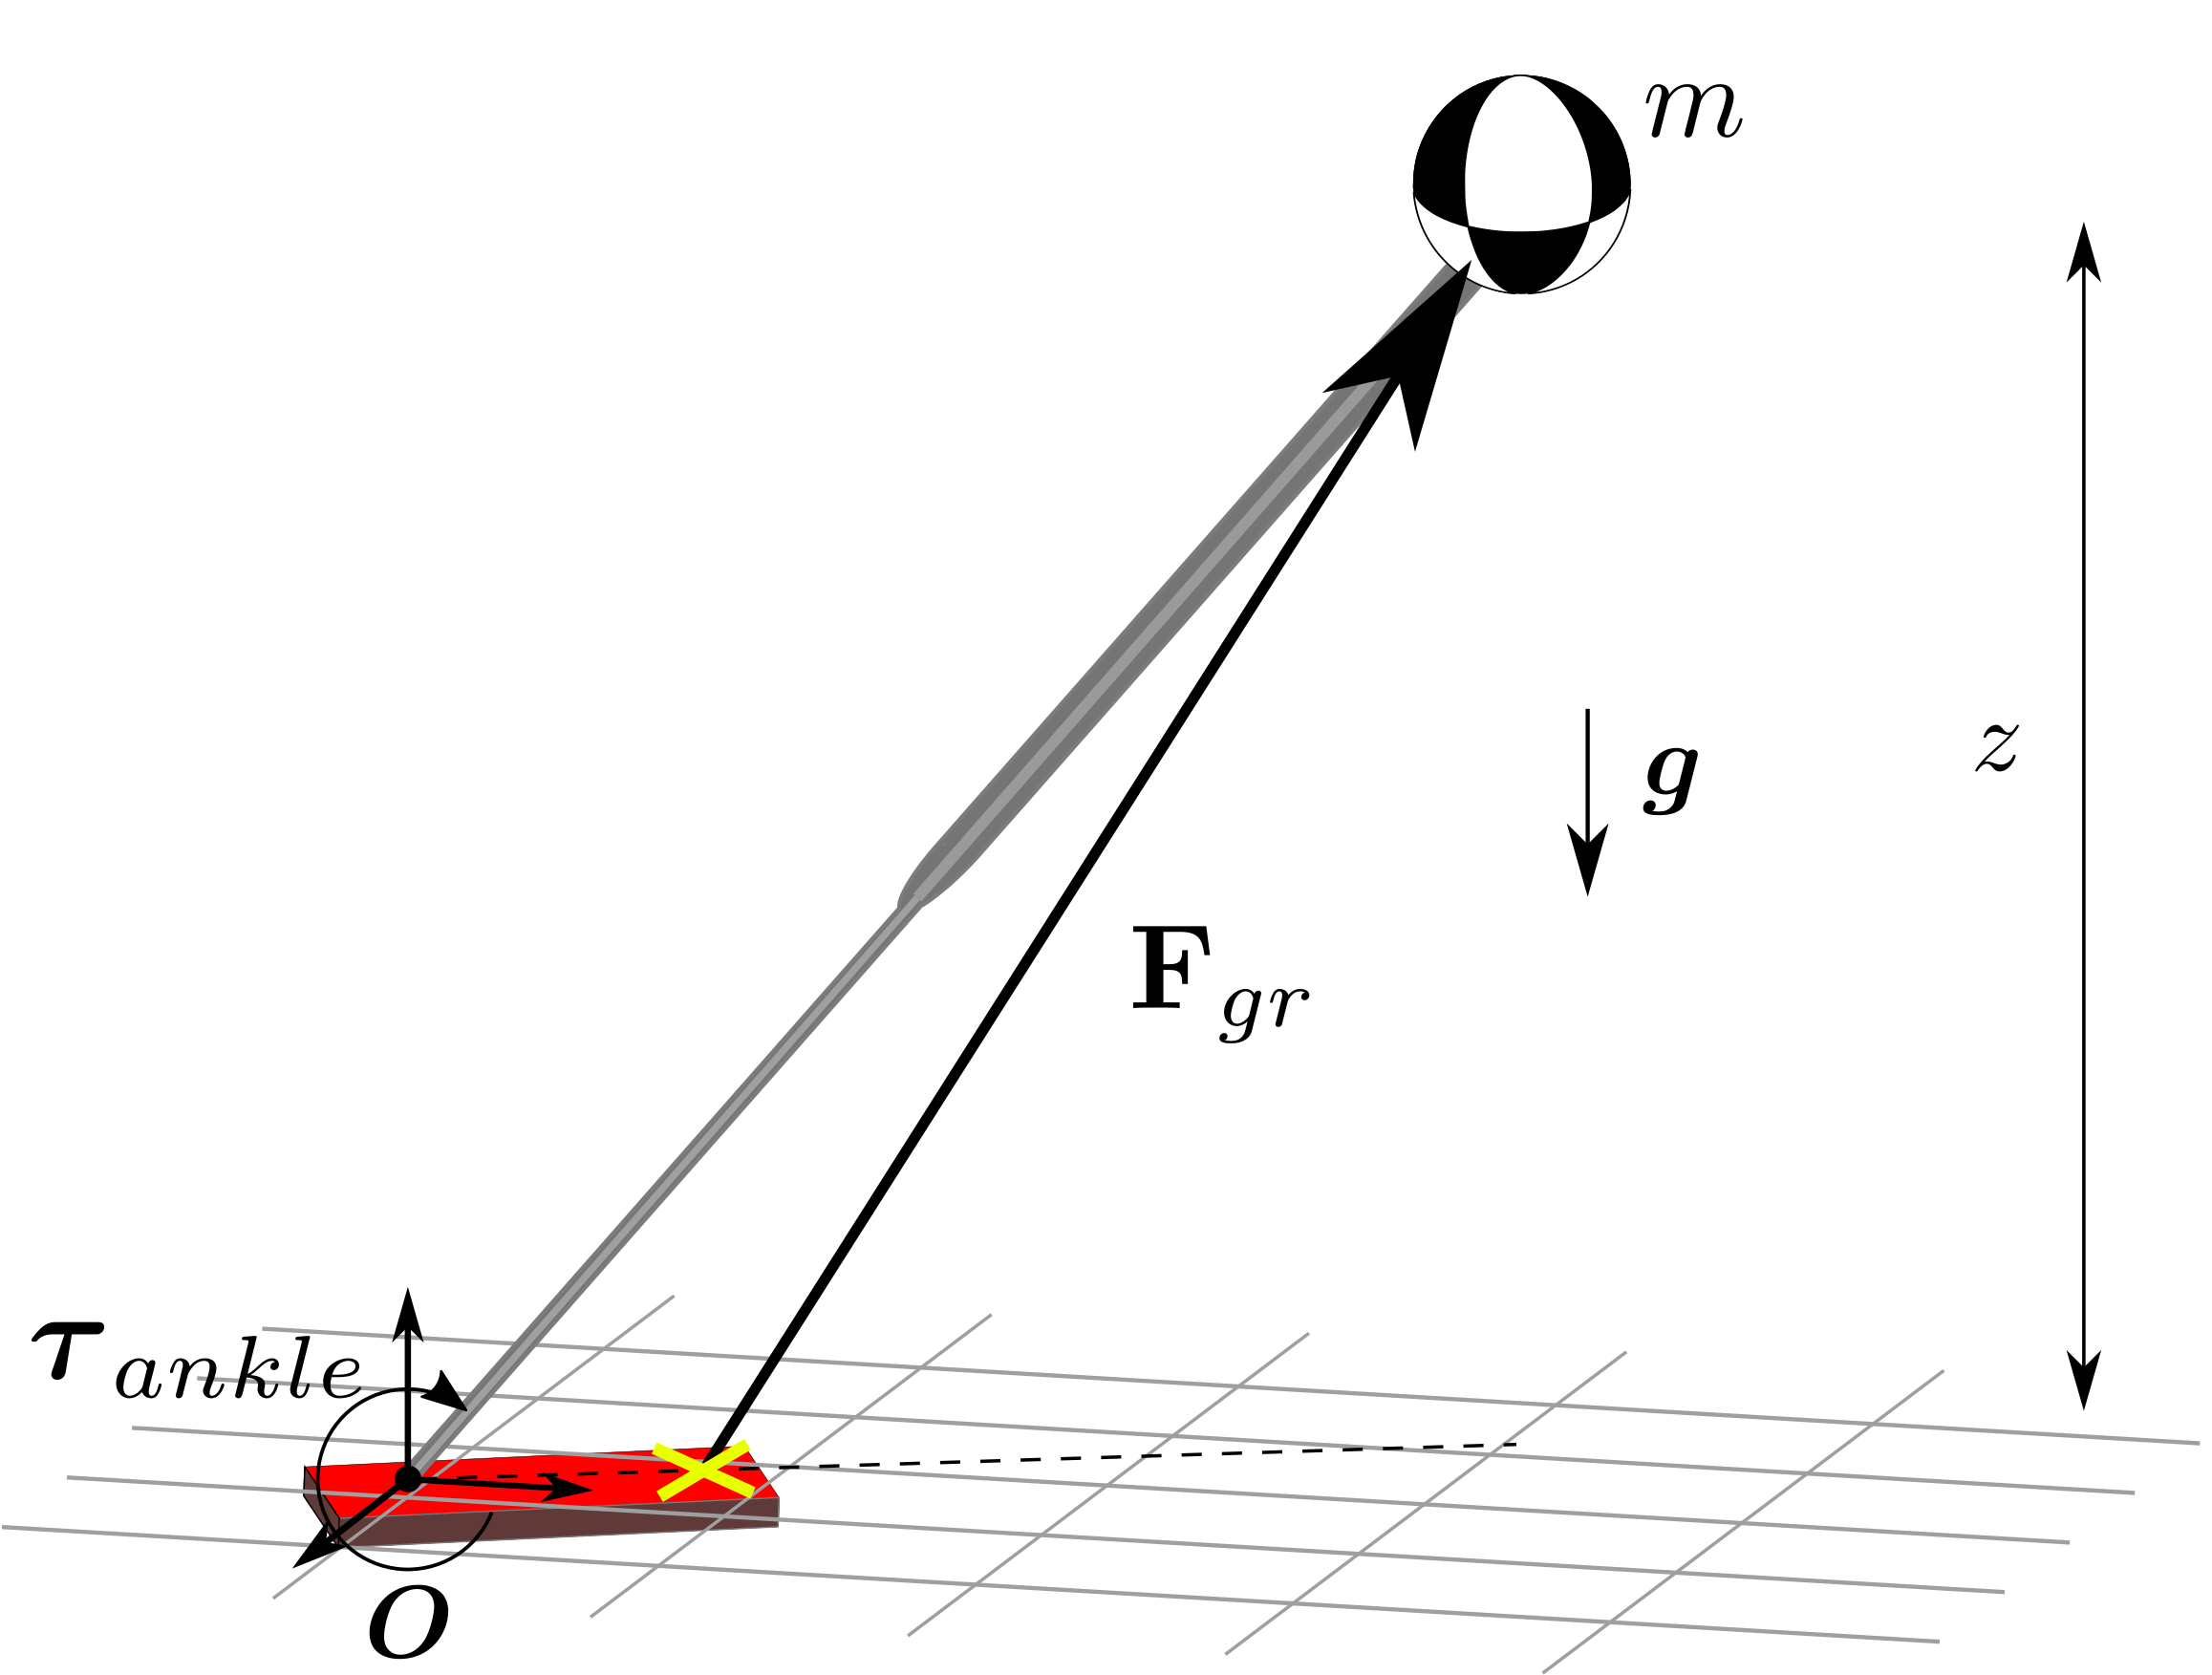
\includegraphics[width=.95\linewidth]{STYLESTUFF/3DCoPviz.png}
\caption{}
\label{fig:3dlipfoot}
\end{subfigure}
\begin{subfigure}{0.49\textwidth}
\centering
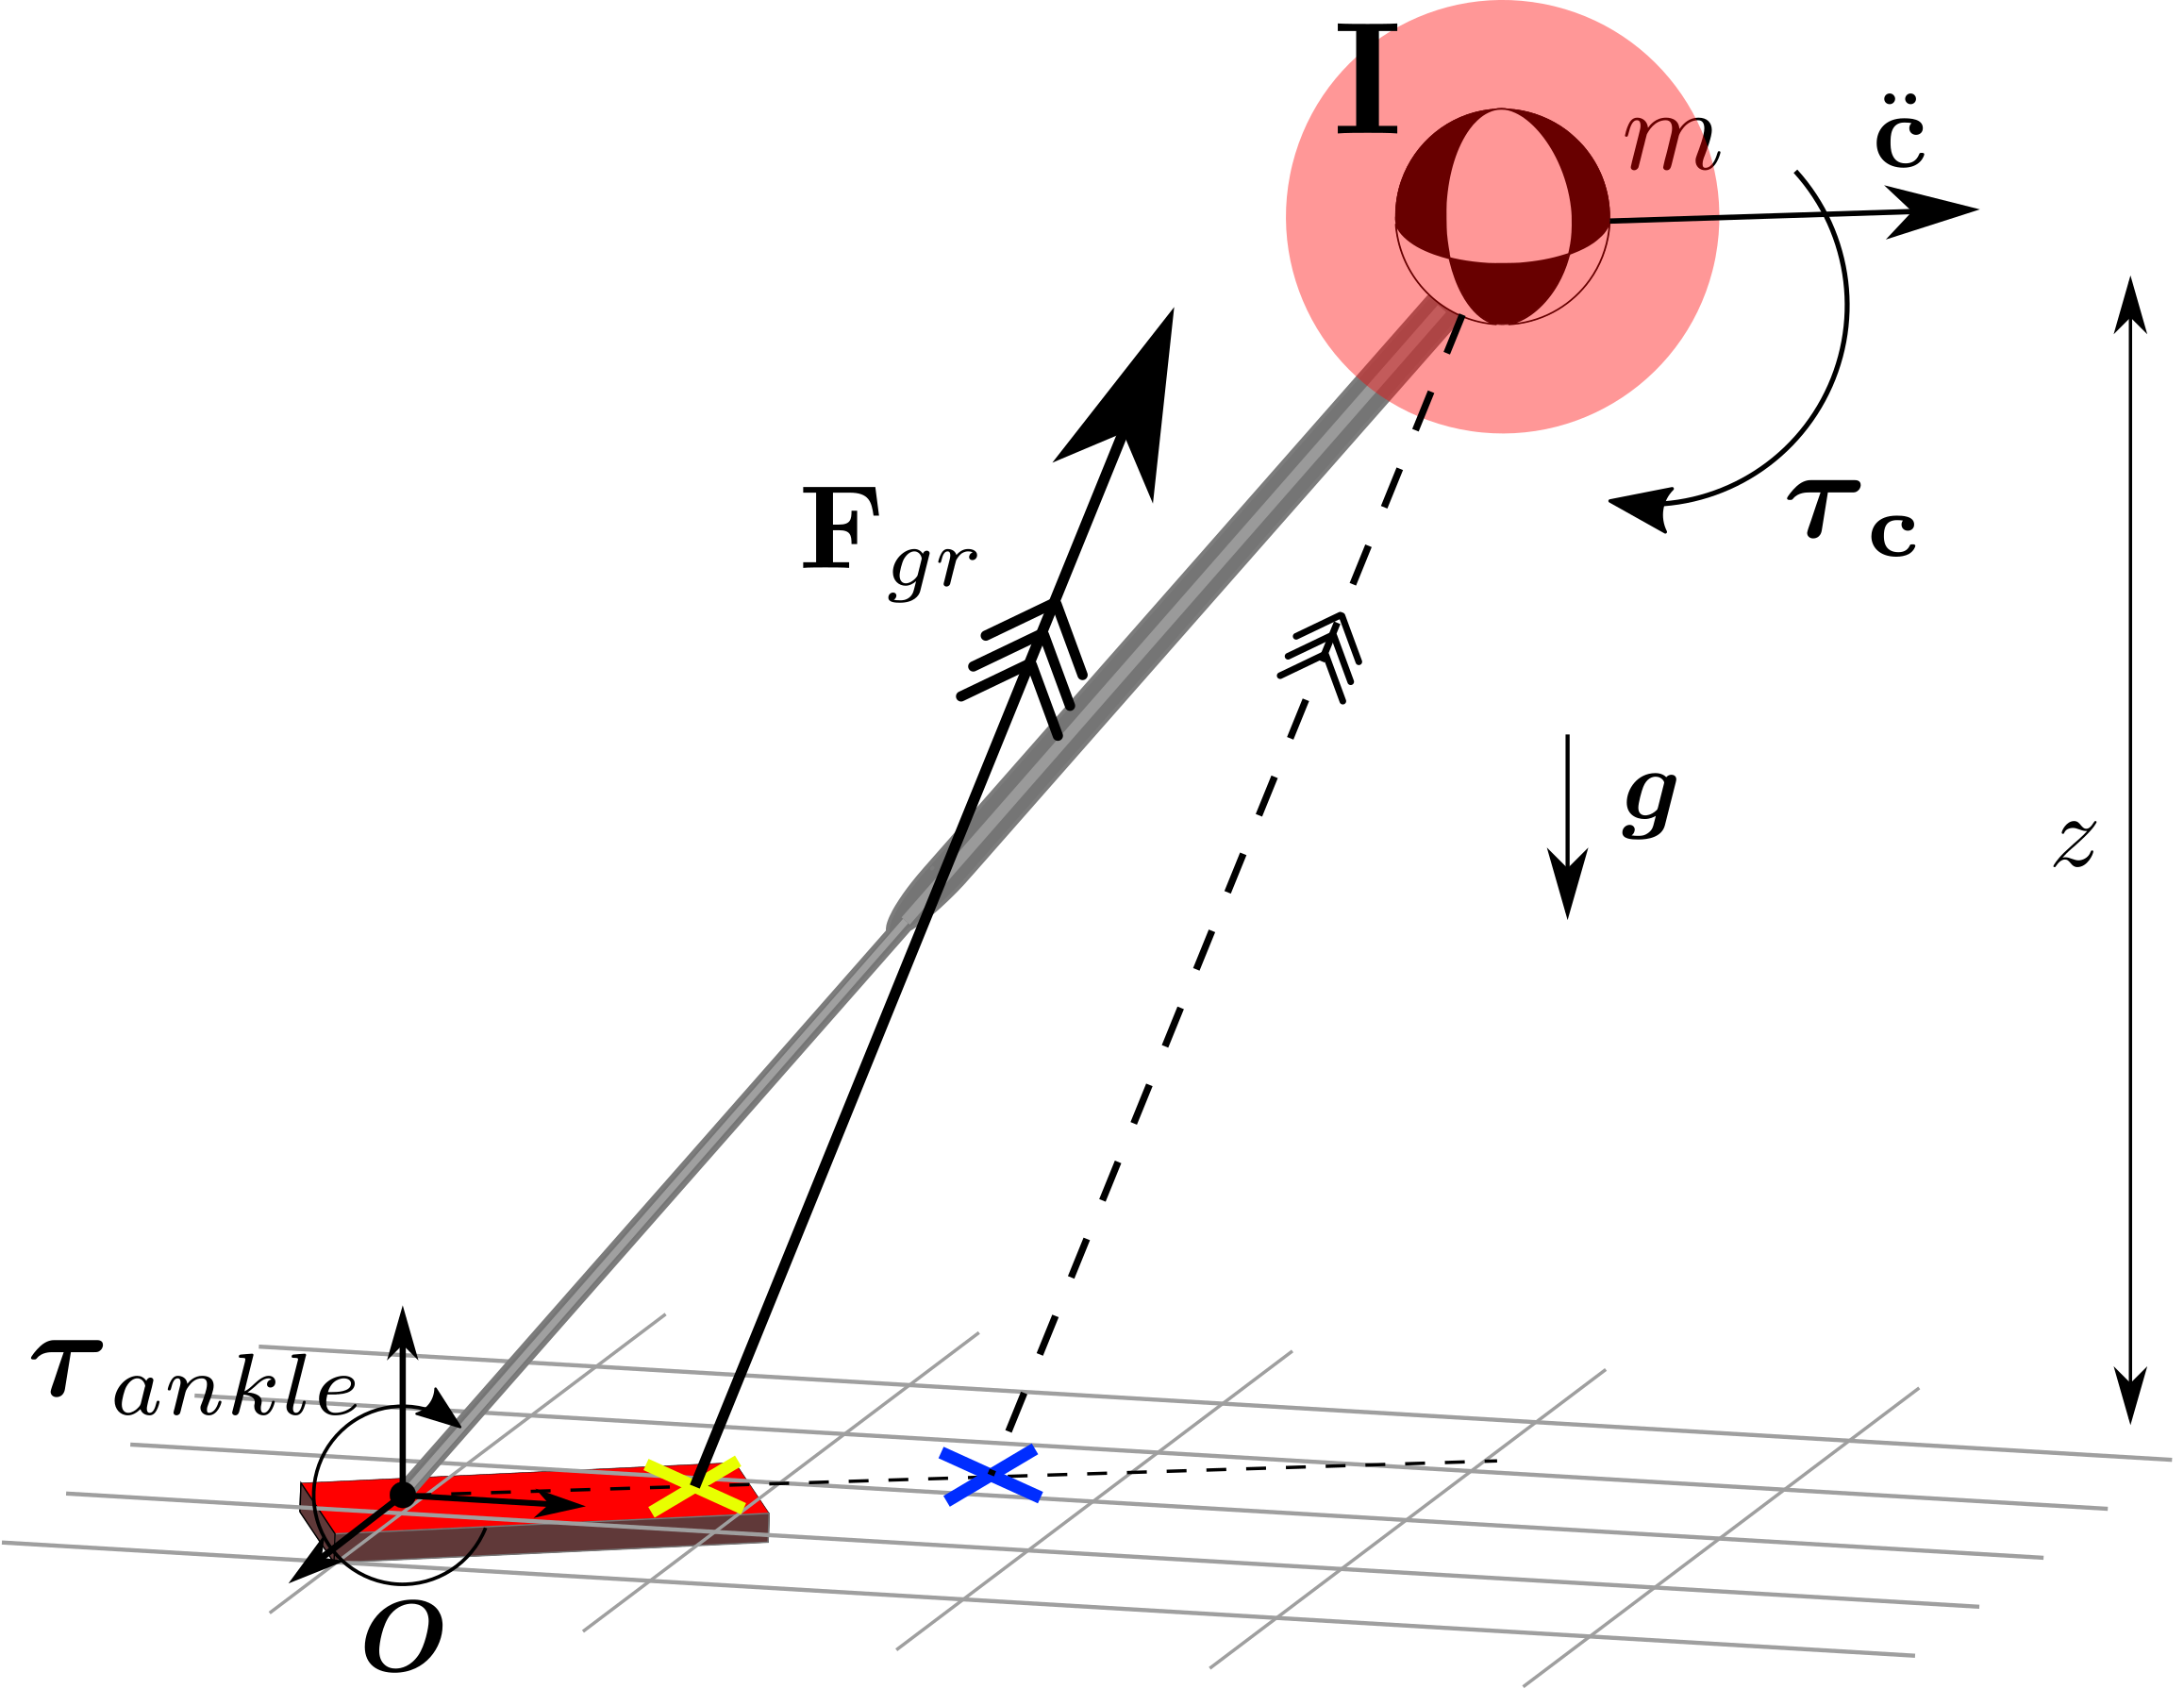
\includegraphics[width=.95\linewidth]{STYLESTUFF/3DCMPCoPviz.png}	
\caption{}
\label{fig:3dlipfootinertia}
\end{subfigure}
\caption{Ground reference points for different modeling choices. (a) The yellow cross points out the \ac{ZMP} location. As no angular momentum is considered in the model, it intersects with the \ac{CMP}. (b) Angular momentum is added to the model, the blue cross points out the \ac{CMP} location and the yellow cross the \ac{ZMP} location.}
\label{fig:zmpvscmp}
\end{figure}


%leg modeling
\subsection{Pendulum-based Models}
The modeling of the leg can subdevided in two categories: the \ac{LIP} model and models that consider \ac{CoM} height variation. \todo{explain that this is virtual leg and not necessarily the prismatic joint as with flywheel model}
\paragraph{The linear inverted pendulum model} is widely used in walking research and especially in robotics \cite{kajita20013d}. In the \ac{2D} \ac{LIP} equations of motion, the motion of the tip along the $x$-axis does not affect the pendulum length $l$:
\begin{equation}
\ddot{x}=\frac{g}{l}x,
\label{eq:LIPeom}
\end{equation}
where $x$ the horizontal location of the pendulum tip and $\ddot{x}$ its acceleration. At any position $x$, a local virtual straight pendulum can be considered, so this motion is at a constant height and $l=z_0$  holds. In \ac{3D}, the system dynamics can be decoupled and the dynamics in $y$-direction read the same: $\ddot{y}=\frac{g}{l} y$. In \figref{fig:3dlip} the \ac{3D} motion is visualized if the \ac{CoM} is relatively far from from the base. The pendulum base lies in the origin and $\cxy = [x,y]^T$ is the \ac{2D} \ac{CoM} projection on the horizontal plane. Because the \ac{LIP} assumption holds, the vertical component of the leg force $\boldsymbol{f}$ has to cancel out gravity acceleration: $f_z=mg$.\\
\begin{figure}[h]
\centering
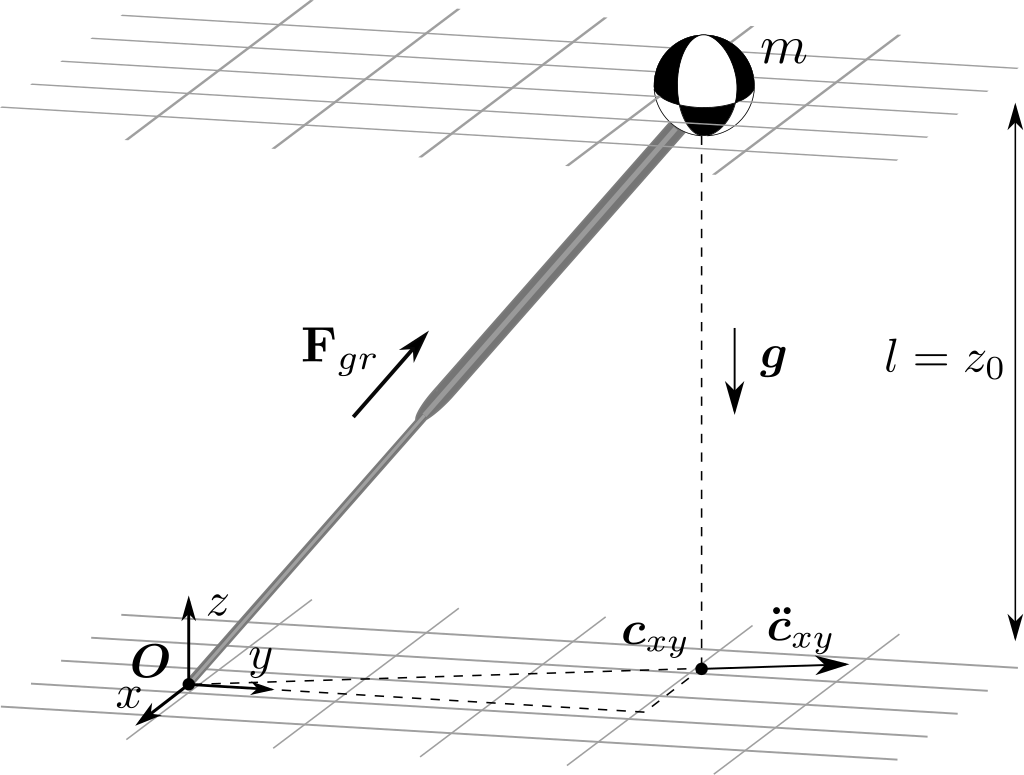
\includegraphics[width=0.5\textwidth]{STYLESTUFF/3DCoMwithoutfoot.png}
\caption{\ac{3D} motion of \ac{LIP} model.}
\label{fig:3dlip}
\end{figure}

% height var model
\paragraph{Height varying models} consider, unlike the \ac{LIP}, height variation of the \ac{CoM}. Three examples of such models are:
\begin{itemize}
	\item The inverted pendulum model \cite{kuo2005energetic}
	\item The \ac{SLIP} model \cite{liu2015trajectory}
	\item A model with prismatic joint: varyable height inverted pendulum \cite{pratt2007derivation}
\end{itemize}
The inverted pendulum model is often used in human motion studies. The \ac{SLIP} model originates from hopping and running robots \cite{schwind1998spring} and models the inverted pendulum as a spring. In \figref{fig:2Dnonlinmodel} the full nonlinear model with pristmatic leg joint is shown in \ac{2D}. The dynamics of the point mass can be written in two ways. One is as a function of the virtual leg force $\vect{f}$:
\begin{equation}
	m\ddot{x} = \vect{f}\frac{x}{\sqrt{x^2 + z^2}}.
	\label{eq:dynamicsprattstyle}
\end{equation}
The other one is as a function of the vertical acceleration $\ddot{z}$:
\begin{equation}
	\ddot{x} = \frac{g+\ddot{z}}{z}x.
	\label{eq:dynamicscaronstyle}
\end{equation}
Note that those models are identical, but can be used for different purposes.
\begin{figure}[h]
\centering
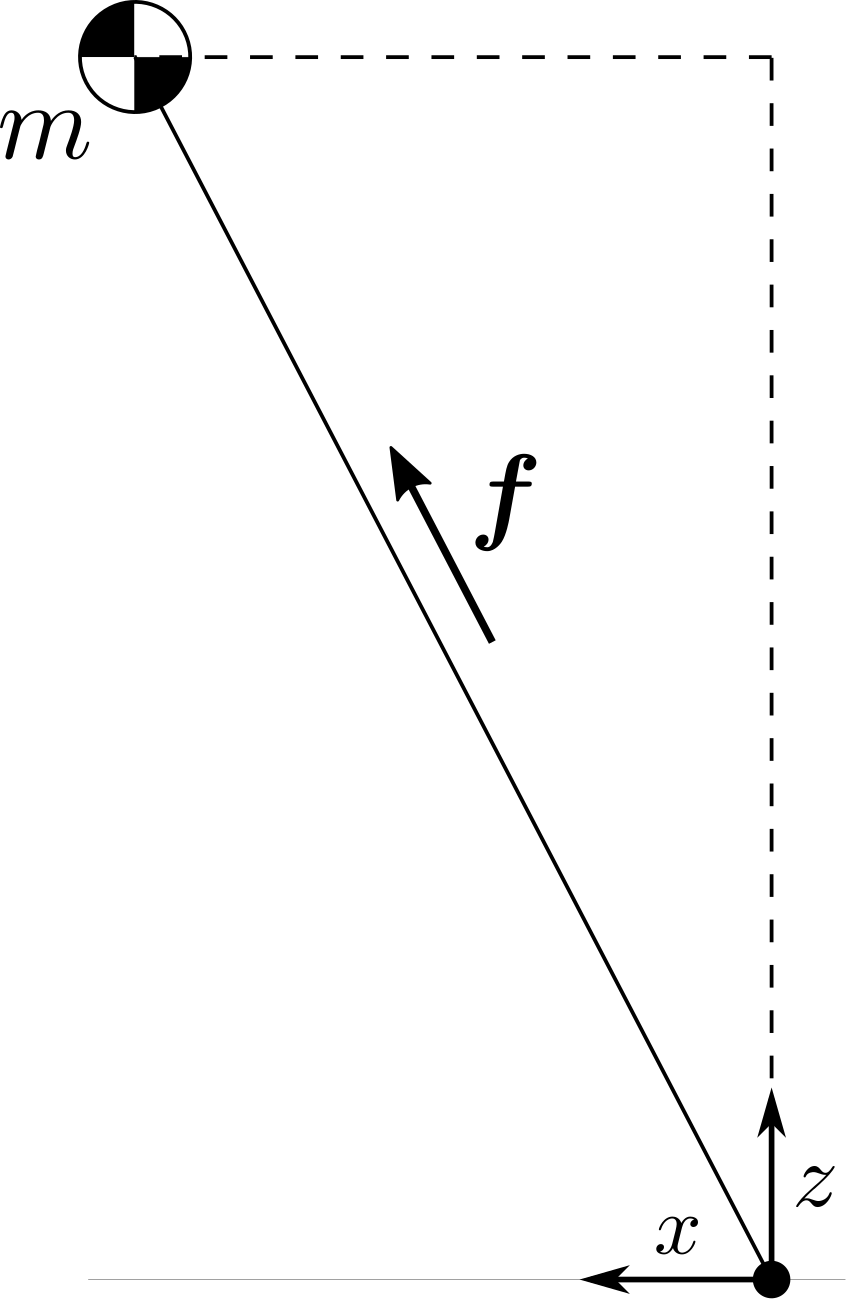
\includegraphics[width=0.2\textwidth]{STYLESTUFF/2Dnonlin.png}
\caption{Basic \ac{2D} inverted pendulum model with varying length.}
\label{fig:2Dnonlinmodel}
\end{figure}

% Energy of Walking
\subsection{Orbital Energy \& Capture}\label{sec:ewalking}
To have an indication of the state on a future moment in time, a form of energy of the system can be derived. With this energy can for example be determined whether or not the current state is stabilizable within the current footstep or coming footsteps: capturability \cite{koolen2012capturability}. 

% LIP orbital energy
\paragraph{The linear inverted pendulum orbital energy}\label{subsec:liporbit} is originally derived in \cite{kajita1992dynamic} and shows another advantage of the use of \ac{LIP} models. For the same reason that force is mass times acceleration: $F=ma$, impuse momentum is force times velocity: $I=Fv$ and the energy or work done by a force is the force times the distance, and thus the impulse integrated over the time interval: $E = Fs = \int Fv dt$, there can be reasoned that if one takes the time integral of the product of the second and the first derivative of a position, an expression for a normalized energy can be achieved: $\frac{E}{m}=\int av dt$. In the mentioned publication that same action is applied on Eq. \eqref{eq:LIPeom}:
\begin{equation}
\Elip = \int (\ddot{x}-\frac{g}{l}x)\dot{x} dt = \frac{1}{2}\dot{x}^2-\frac{g}{2z_0}x^2 +C=0
\label{eq:Elip}
\end{equation}
with $C$ the integration constant. The \ac{LIP} orbital energy is defined as $E_{LIP}=-C$. If $E_{LIP}>0$, the point mass will cross the $x$ position of the pendulum base with its current velocity. If $E_{LIP}<0$, the point mass will not cross the pendulum base and will have a turning point where the velocity becomes zero.

% ICP
\paragraph{The instantaneous capture point} is an extention of the \ac{CP}, which is derived more than a decade later from $\Elip$ in \cite{pratt2006capture}. Taking $E_{LIP}=0$ and taking the square root of Eq.  \eqref{eq:Elip} gives
\begin{equation}
x_{cp}=\sqrt{ \frac{z_0}{g}}\dot{x} 
\label{eq:cp}
\end{equation}
where $x_{cp}$ is the \ac{CP}, based on the current tip velocity $\dot{x}$. This is the point where the velocity is exactly driven to zero and the pendulum is upright, where neither crossing of the pendulum base ocurred nor turning of body velocity. In \figref{fig:2dicp} a \ac{2D} visual explanation is given of this point.
\begin{figure}[h]
\centering
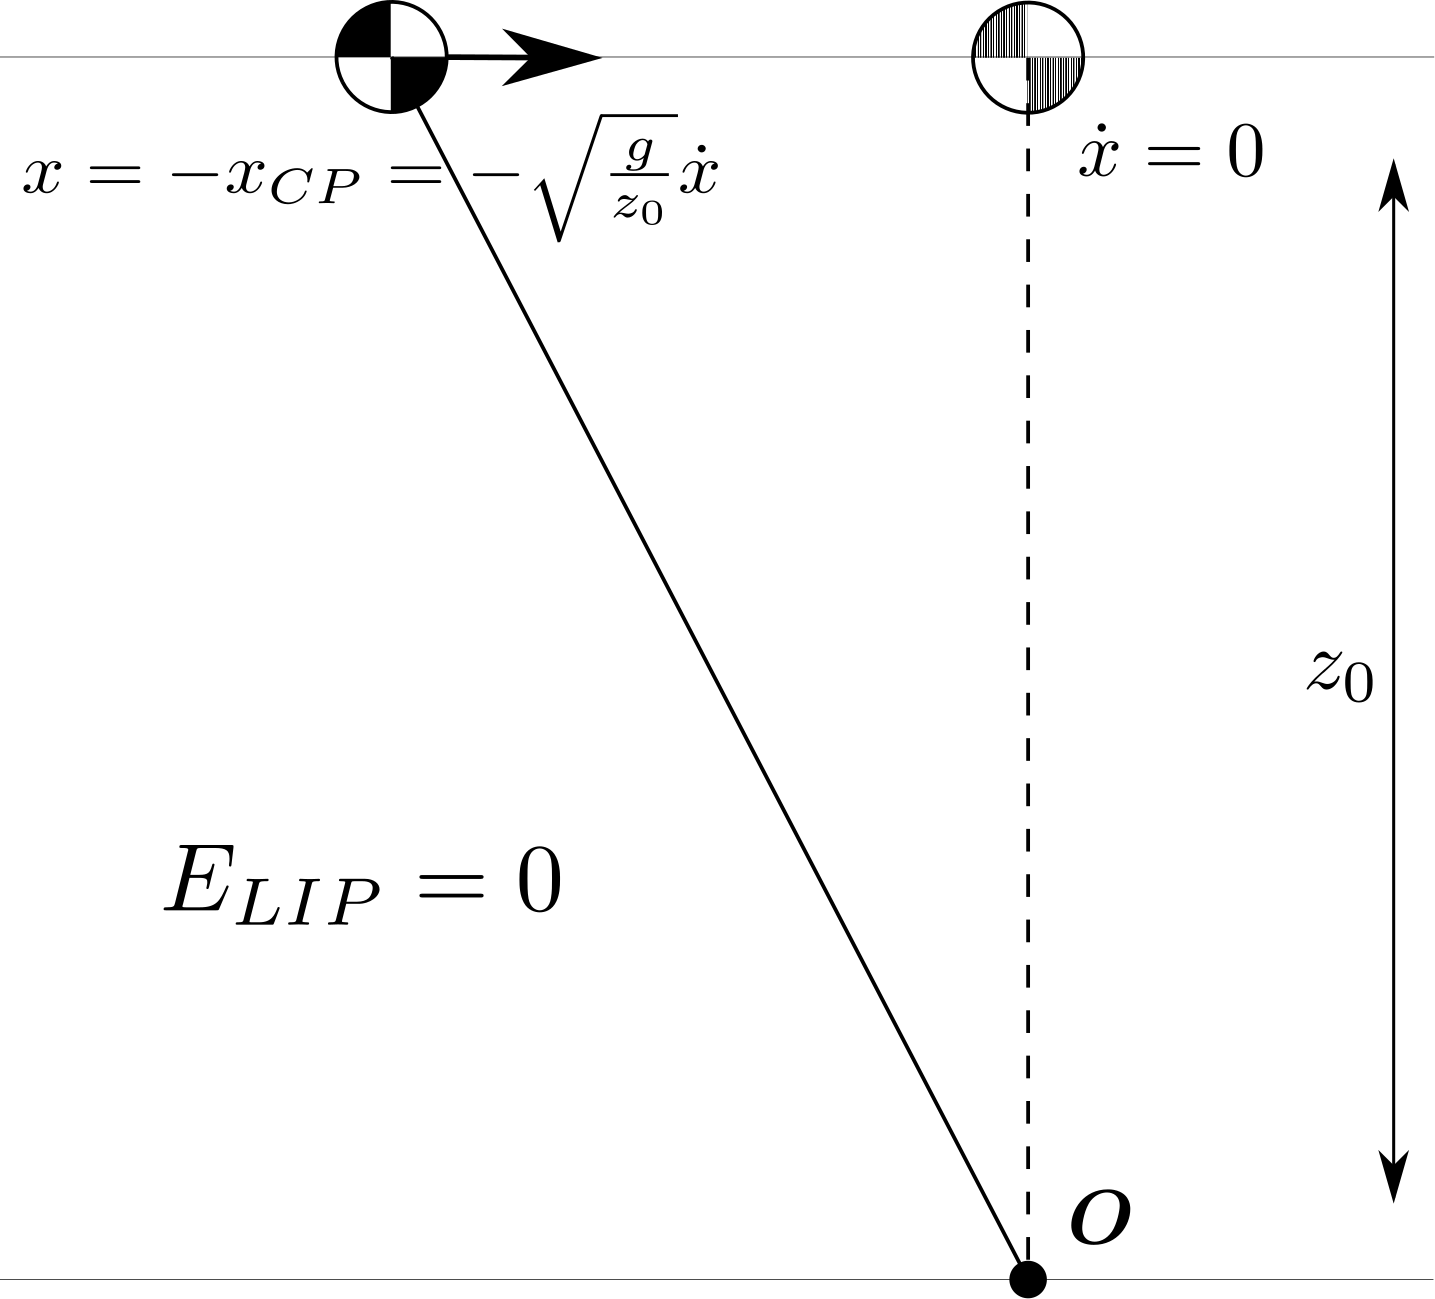
\includegraphics[width=0.4\textwidth]{STYLESTUFF/2DICP.png}
\caption{Visualization of the path to the \ac{CP}. }
\label{fig:2dicp}
\end{figure}
\paraskip
Later, the \ac{ICP} was introduced \cite{koolen2012capturability}, which gives a slightly different discription of the point:
\begin{equation}
\icpx=x+\sqrt{ \frac{z_0}{g}}\dot{x} 
\label{eq:icp}
\end{equation}
where $\icpx$ is the \ac{ICP}. In this way, the point can be described in the environment coordinates and can be seen as a point where to step in the environment to come to a stop.
The $x$- and $y$-coordinate can be decoupled as in the equations of motion of Eq. \eqref{eq:LIPeom}. However, in \ac{3D}, convergence to the capture point in one direction does not also include convergence to the capture point in the other, as the direction of motion can also be directed not towards the pendulum base. Other similar mentions to the \ac{ICP} are extrapolated center of mass \cite{hof2008extrapolated} and the \ac{DCM} \cite{takenaka2009real}. 
\paraskip
For modeling and planning the time derivative is taken of the \ac{ICP}: the \ac{ICP} dynamics \cite{koolen2012capturability}. This time derivative can be written as a function of the current \ac{ICP} location and a ground reference point:
\begin{equation}\label{eq:icpdyn}
\dot{\icp}=\sqrt{ \frac{g}{z_0}}(\icp-\rcmp)
\end{equation}
where $\icp$ is the \ac{2D} vector of the \ac{ICP} location and $\rcmp$ the \ac{2D} \ac{CMP} location. The choice of a ground reference point depends on modeling choices, like inclusion of angular momentum for example.

% Boundedness
\paragraph{The boundedness condition} \cite{lanari2014boundedness} includes the effects of the motion of the ground reference point in the capture problem and approaches the capture problem from a perspective that the point-mass has to converge to zero velocity in finite time. The solution of $x_u$, a point that also coincides with the \ac{ICP}, reads as:
\begin{equation}
x_u(t,r) = e^{\omega_0(t-t_0)}x_u(t_0) -\omega_0 \int_{t_0}^t e^{\omega_0(t-\tau)}r(\tau)d \tau,
\end{equation}
where $r(t)$ is the trajectory described by the used ground reference point, the virtual base of the pendulum. The boundedness condition reads as follows: if the the future input $r(t)$ makes the system converge, the following equality holds:
\begin{equation}
x_u(t_0) = \omega_0 \int_{t_0}^{\infty} e^{-\omega_0(\tau-t_0)}r(\tau)d \tau.
\end{equation}
The initial condition, which is equal to the \ac{ICP}, has to be related to $r(t)$ by this expression.

%nonlinear orbital
\paragraph{Orbital energy with height variation}\label{subsec:nonorbit} is a more difficult to derive than its linear counterpart.  Examples of attempts to include \ac{CoM} height variations in the solution to the dynamics are the time-varying \ac{DCM} \cite{hopkins2014humanoid}, the orbital energy under a virtual constraint \cite{pratt2007derivation} and the height varying boundedness condition \cite{caron2018balance}. These works are discussed in the Section 
\ref{sec:relatedworksheight}, since they are highly related to the research of focus.

% Control Framework IHMC
\section{Humanoid Robotics at IHMC}
To support the theory discussed in later experiments, in this chapter a brief background of humanoid robotics at \ac{IHMC} is given. Almost all algorithms are written in Java and similutations are run in \ac{SCS}.
%robots
\subsection{Robots}
At the moment of writing, there are two humanoid robots present at the institute, Boston Dynamics' Atlas and NASA's Valkyrie. An important difference between the two robot is that Atlas is hydraulically actuated, while Valkyrie relies on electric series elastic actuators. An advantage of the use of hydraulic acuation is the capability of reaching high torques. Series elastic actuators on the other hand are generally better for torque sensing. In \figref{fig:robots} the two robots are shown.
\begin{figure}[h]
\centering
  \begin{subfigure}{0.45\textwidth}
  \centering
  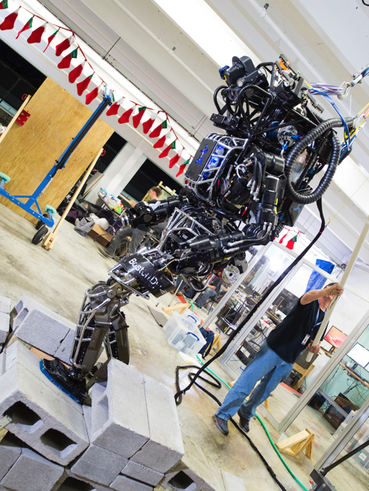
\includegraphics[width=.8\linewidth]{STYLESTUFF/AtlasOld.png}
   \caption{}
    \label{fig:atlas}
  \end{subfigure}
  \begin{subfigure}{0.45\textwidth}
    \centering
  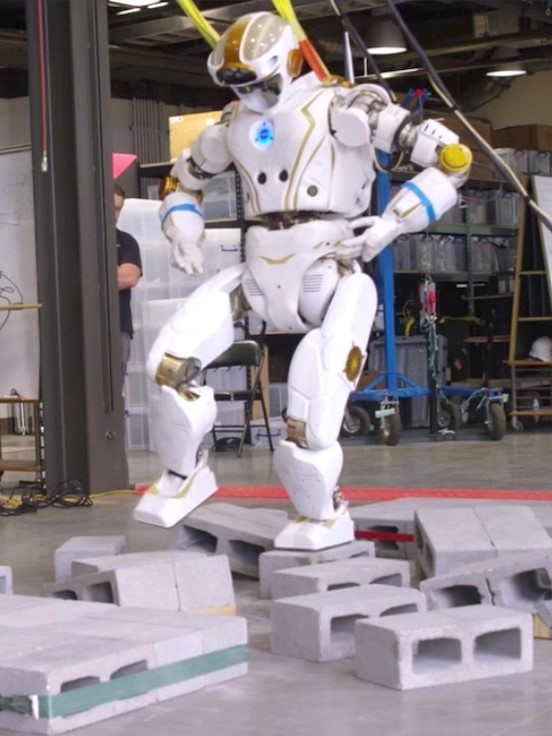
\includegraphics[width=.8\linewidth]{STYLESTUFF/Valkyrie.jpeg}
  \caption{}
   \label{fig:valkyrie}
  \end{subfigure}
  \caption{(a) Atlas \cite{oldatlas} and (b) Valkyrie \cite{valkyrie} walking over an un-even cinder block field at IHMC }
  \label{fig:robots}
\end{figure}
%walking states
\subsection{Walking States}
In contrary to running, with walking there is a state in every cycle with two feet in contact with the ground. This is the \ac{DS} state and the state where only one leg is on the ground is the \ac{SS} state. In \ac{SS}, the leg in contact with ground is the support leg and the foot taking a step is the swing leg. The transition between those states and the duration in each state play an important role in the generation of a dynamic plan and in the control framework. For example, in the control framework state transitions initiate the start a new trajectory or motion objective for one of the feet.
% planning
\subsection{Planning}
Planning of the robots motion in space is executed by seperating footstep planning from the generation of a dynamic plan. The dynamic plan is in this case an \ac{ICP} plan, but this is only one of the methods that exist in the field of research.
%footstepplan
\paragraph{Footstep planning} is the generation of a sequence of footsteps for the robot to follow. A \ac{LiDAR} sensor on the head of the robot provides terrain information. One way to generate a footstep plan is to let the user define it via a \ac{GUI}. Via relatively simple algorithmic checks on for example kinematic reachability, the \ac{GUI} can show whether a to be placed footstep is feasible or not. To make this process more autonomous, recently developments have been made in the creation of a footstep planner based on a A* search algorithm. 
%icpplanning
\paragraph{Instantaneous capture point planning}\label{subsec:icpplan} is the generation of a dynamic plan for the robot. It relies on the solution of the linear differential equation the \ac{ICP} dynamics of \eqref{eq:icpdyn}:
\begin{equation}\label{eq:icpsol}
	\icp(t)=e^{\omega_0t}(\icp_0- \vect{r}) + \vect{r},
\end{equation}
where $\vect{r}$ is the virtual point-foot location, $\omega_0=\sqrt{\frac{g}{z_0}}$ is the natural frequency of the \ac{LIP} and $\icp_0$ is the initial \ac{ICP} location. This equation is only valid if the location of the virtual point-foot is assumed to be constant. The virtual point-foot depends on the model considered, but is typically the \ac{ZMP} or \ac{CoP} when no angular momentum is considered and the \ac{CMP} when an attempt is made to estimate the amount of angular momentum generated by the walking motion. 
\paraskip
Under the assumption of the constant virtual point-foot locations, multiple methods have been developed over the years and improvements are still going on. The most traditional generation of a \ac{ICP} reference trajectory is calulated with a single \ac{ZMP} knotpoint \cite{englsberger2012integration}. Using this method, for every footstep a single \ac{ZMP} knotpoint is used, and \ac{ICP} knotpoints $\icp_{0,n}$ for the $n$-th step are calculated by integrating the \ac{ICP} dynamics backwards in time for the footsteps considered. Using \eqref{eq:icpsol}, the local \ac{ICP} refence value can be computed at any time instance within the plan. 
\paraskip
The above mentioned method is improved in \cite{englsberger2014trajectory}, where multiple \ac{CMP} knotpoints per foot are considered and \ac{SS} and \ac{DS} transitions are interpolated using splines. In the most recent improvements, continous \ac{CMP} reference trajectories are used for the generation of the \ac{ICP} trajectory \cite{seyde2018inclusion}. An estimate of the angular momentum generated during the walking motion is incorporated in the generation of the \ac{CMP} reference. At the time of writing, the latter method is the one currently in use, and which is used for the experiments in this thesis.
% icp control
\subsection{Instantaneous Capture Point Control}
From an \ac{CMP} and \ac{ICP} reference trajectory, the following control law is used to generate a desired \ac{CMP}:
\begin{equation}
    \rcmpd=\rcmpr + \mathbf{k}_{\xi}(\icp-\icpr),
    \label{eq:rcmpd}
\end{equation}
where $\rcmpd$ is the desired \ac{CMP}, $\rcmpr$ and $\icpr$ are the reference \ac{CMP} and \ac{ICP} from the \ac{ICP} planner respectively and $\icp$ is the current \ac{ICP}. From $\rcmpd$, the desired horizontal linear momentum rate of change can be computed:
\begin{equation}\label{eq:dotldxy}
    \dotldxy = \frac{\cxy-\rcmpd}{z_0}mg,
\end{equation}
where $\dotldxy$ is the desired horizontal linear momentum rate of change, which is basically the desired horizontal force. This value is send to the momentum-based control framework. 

% momentum control
\subsection{Momentum-based Whole-body Control}
The desired horizontal linear momentum rate of change $\dotldxy$ from \ac{ICP} control is one of the inputs for the the whole-body \ac{QP}. The the solution of the whole-body \ac{QP} goes into a inverse dynamics solver, which calculates desired joint torques. 
%centroidal
\paragraph{Centroidal dynamics} \cite{orin2013centroidal} translate joint states to state on and around the \ac{CoM}. The  mapping between joint velocities and end-effector motion plays a crucial role in any robotic system:
\begin{equation}\label{eq:jacobian}
\matr{T}=\begin{bmatrix}\bs{\omega} \\ \bs{\upsilon} \end{bmatrix} = \matr{J}(\qjnt)\dqjnt \in \mathbb{R}^6,
\end{equation}
where $\dqjnt$ are the joint velocities, $\matr{J}(\qjnt)$ is the Jacobian that maps joint velocities to the end-effector twist$\matr{T}$. The twist consist of the angular velocity $\bs{\omega} \in \mathbb{R}^3$ and the linear velocity $\bs{\upsilon} \in \mathbb{R}^3$. In humanoid robotics, a fairly common approach is the use of centroidal momentum:
\begin{equation}
\vect{h}=\begin{bmatrix}\vect{k} \\ \vect{l} \end{bmatrix} =\matr{A}(\qjnt)\dqjnt,
\end{equation}
 where $\matr{A}=\matr{I}\matr{J}$ is the inertia matrix $\matr{I}$ times the jacobian. The centroidal momentum $\vect{h}$ consists of the angular part $\vect{k}$ and the linear part $\vect{l}$. The time derivative of the centroidal momentum plays a crucial part in the control framework currently in use \cite{koolen2016design}:
\begin{equation}
\dot{\vect{h}}=\begin{bmatrix}\dot{\vect{k}}\\ \dot{\vect{l}} \end{bmatrix} =\matr{A}\ddot{\vect{q}} +\dot{\matr{A}}\dot{\vect{q}} = \matr{W}_g + \sum_i\matr{W}_{gr,i} + \sum_i \matr{W}_{ext,i}, 
\end{equation}
where $\matr{W}_g$ is the gravitational wrench and $\sum_i\matr{W}_{gr,i}$ the wrench exterted by \ac{GRF}. The other external wrenches, which can be caused for example by other contacts than ground, are considered zero in this thesis: $\sum_i \matr{W}_{ext,i}=\vect{0}$.
%qp
\paragraph{The whole-body quadratic program} \cite{koolen2016design} that translates momentum objectives, motion objectives and privileged configuration objectives to desired joint accelerations and desired \ac{GRF} is structured as follows:
\begin{equation}
\begin{array}{rlcl}
\displaystyle \min_{\bs{\ddot{q}}_d,\bs{\rho}} & \multicolumn{3}{l}{J_{\bs{\dot{h}}_d} + J_{\bs{J}} + J_{\bs{\rho}} + J_{\bs{\ddot{q}}_d}  + J_p} \\
\textrm{s.t.} & \matr{A}\ddqjntd + \dot{\matr{A}}\dqjnt = \matr{W}_g + \matr{Q}\bs{\rho}+\sum_i\matr{W}_{ext,i}\\
&\displaystyle \bs{\rho}_{min} \leq \bs{\rho}\\
&\ddot{\qjnt}_{min} \leq \ddqjntd \leq \ddot{\qjnt}_{max},
\end{array}
\end{equation}
where $\ddqjntd$ are the desired joint accelerations, $\matr{Q}\bs{\rho} = \sum_i\matr{W}_{gr,i}$ is the basis vector matrix $\matr{Q}$ times the basis vector multipliers $\bs{\rho}$. In \figref{fig:wrenchcone}, the basis vectors are visually explained.  
\begin{figure}[h]
\centering
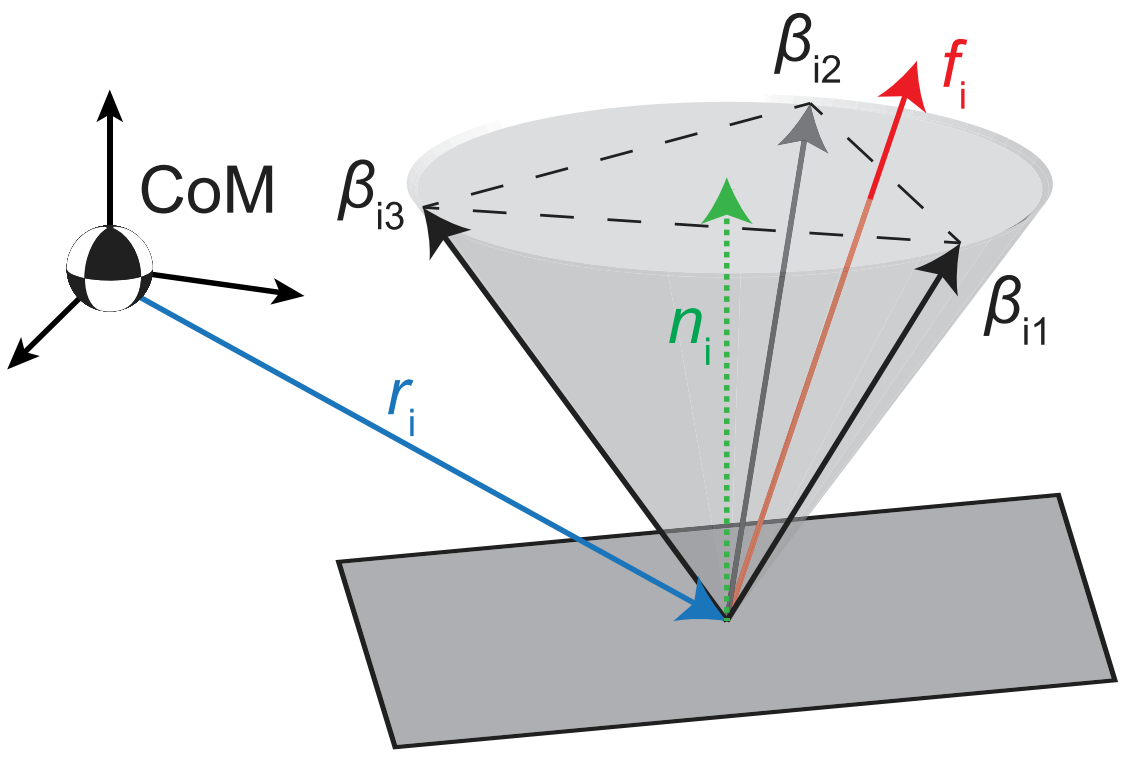
\includegraphics[width=0.4\textwidth]{STYLESTUFF/wrenchcone.png}
\caption{Wrench cone with basis vectors \cite{koolen2016design}. }
\label{fig:wrenchcone}
\end{figure}
The minimum $\bs{\rho}_{min}$ has to be at least zero, because of the unilateral contact constraint of the robot. The total cost $J$ is composed of the following cost terms:
\begin{equation*}
\begin{array}{rlcl}
$Momentum objective cost:$ & J_{\dot{\vect{h}}_d}= \wght_{\dot{\vect{h}}_d}||\matr{A}\ddqjntd + \dot{\matr{A}}\dqjnt - \dot{\vect{h}}_d||^2\\
$Motion objective cost:$ & J_{\matr{J}_m} = \wght_{\matr{J}_m}||\matr{J}_m\ddqjntd-\vect{p}||^2\\
$Contact force cost:$ & J_{\bs{\rho}}=\wght_{\bs{\rho}}||\bs{\rho}||^2 \\
$Joint acceleration cost:$ & J_{\ddqjntd} = \wght_{\ddqjntd}||\ddqjntd ||^2 \\
$Privileged configuration cost:$ & J_p = \wght_p||(\matr{I} - \matr{J}_t^{\dagger}\matr{J}_t)\ddqjntd - \ddqjntp||^2,
\end{array}
\end{equation*}
where the weighting terms $\wght$ can have a selecting function as well. For example the centroidal momentum rate of change objective $J_{\dot{\vect{h}}_d}$ only consists of the linear part and is only affected by $\dotld$. The motion task jacobian $\matr{J}_m = [\matr{J}_1^T\quad...\quad\matr{J}_N^T]^T$ and objective vector $\vect{p} = [\vect{p}_1^T\quad...\quad\vect{p}_N^T]^T$ consist of all concatenated jacobians and objective values that map either joint acceleration to end-effector motion, as in Equation \eqref{eq:jacobian} or joint acceleration to joint joint acceleration. The motion objective values $\vect{p}$ consist of PD-controlled desired accelerations, coming for example from trajectory tracking of the swing leg or maintaining the upper-body orientation. The last cost term $J_p$ is determined by the privileged joint accelerations $\ddqjntp$. Here is $\matr{J}_t$ the all-task jacobian consisting of both $\matr{A}$ and $\matr{J}_m$. The damped Moore-Penrose pseudo-inverse  $\matr{J}_t^{\dagger} = \matr{J}_t^T(\matr{J}_t\matr{J}_t^T +\mu^2)^{-1}$ with $\mu>0$ is used in the null-space projector $(\matr{I} - \matr{J}_t^{\dagger}\matr{J}_t)$, which projects the priviliged acceleration objective in the null-space of the primary task jacobian $\matr{J}_t$. This can for example be used in singularity avoidance, where the priviliged accelerations are used to determine the configurarion of the robotic chain.  
\paraskip
An important note considering the research goal is the generation of vertical \ac{CoM} motion of the robot. The desired linear momentum rate of change $\dotld$ consists, next to its horizontal component of Equation \eqref{eq:dotldxy}, of a vertical part:
\begin{equation}
\dotldz =m(k_p(z-z_r) + k_d\dot{z}), 
\end{equation}
where $k_p, k_d$ are the PD-control gains and $z_r$ is the reference height coming from a reference trajectory. Decision variables for this trajectory are for example kinematic reachability and height changes in terrain, but maintaining the robot's balance is \textit{not } a part of those decision variables.


\paragraph{Inverse dynamics} translate joint and end-effector states to joint torques. Desired joint torques $\bs{\tau}_d$ are calculated via a revursive Newton-Euler algorithm using solution of whole-body \ac{QP}: $\ddqjntd$ and $\bs{\rho}$.
\begin{equation}
    \bs{\tau}_d = \matr{M}(\qjnt)\ddqjntd + \matr{C}(\qjnt,\dqjnt) + \matr{G}(\qjnt) + \matr{J}^T \vect{W}_{gr},
\end{equation}
where the ground reaction wrench $\vect{W}_{gr}$ is computed with $\bs{\rho}$. A high-level overview of the control framework is shown in \figref{fig:framework}.
\begin{figure}[h]
\centering
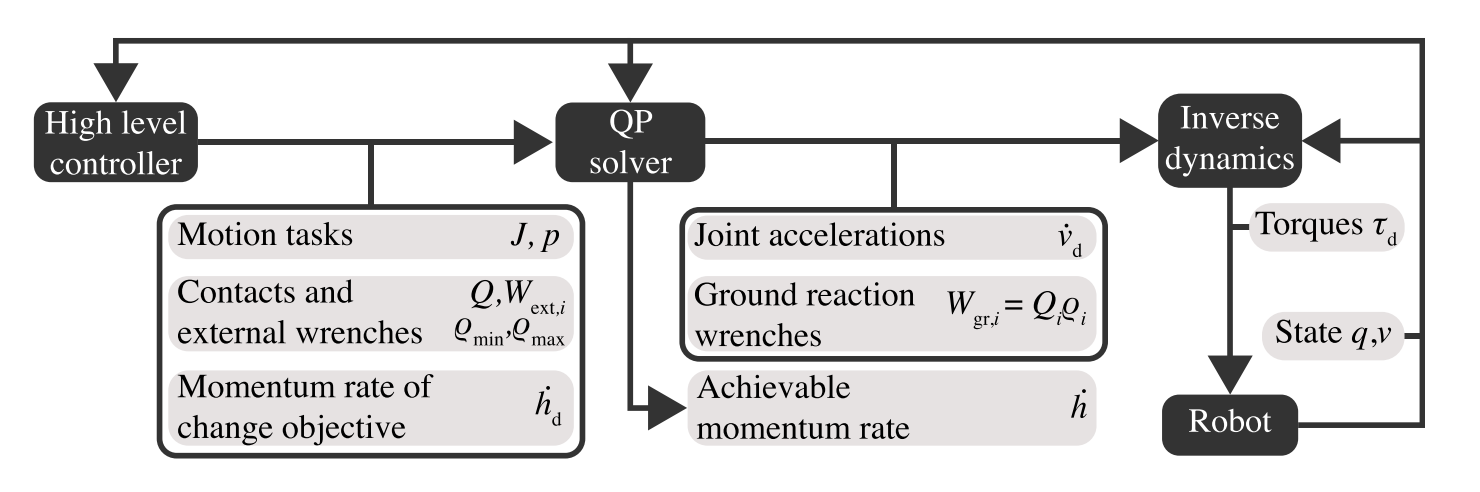
\includegraphics[width=0.8\textwidth]{STYLESTUFF/controlframework.png}
\caption{High-level overview of control framework \cite{koolen2016design}. }
\label{fig:framework}
\end{figure}

% CoM Height Variation
\section{Related Works}\label{sec:relatedworksheight}
To group related works to the study of additional \ac{CoM} height variation compared to the \ac{LIP} model a high level division can be made based on different goals or objectives why vertical \ac{CoM} motion should be considered. As a baseline, objectives are grouped in the following strategies. 

Traditionally, vertical motion is generated through non-predictive control: a dynamic reference plan exists, often based on the LIP model, and height variation are often disturbances on the model considered in the dynamic plan. Reasons to use height variations here include the guarantee of \textit{kinematic feasibility}: height variation allows the robot to step up platforms, and allows the robot to take larger steps. A noteworthy, more unique, example of height variation in non-predictive control is walking with straighter legs as in \cite{griffin2018straight}. The motivation here is to let the robot walk more \textit{human-like}, which could have more underlying benefits, such as kinematic reachability and metabolic energy consumption \cite{wang2012optimizing}.

Because the constant height assumption from the \ac{LIP} is constraining its dynamics, efforts have been made to incorporate CoM height variation in the generation of a dynamic plan. Instead of using an LIP model, a more complicated model is used. \textit{Expected} height variations of the CoM can be incorporated in the dynamic planning problem, which improves the \textit{dynamic feasibility} of the plan. In theory, the reference dynamics are closer to the real dynamics of the robot. Expected height variations from a walking pattern can be received from for example a reference trajectory over an height-varying terrain, or from a human-like walking pattern. 

A very recent objective is the specific use of height variation in \textit{balance control}. Normally, traditional balance control strategies are taking a step, movement of the \ac{CoP}: `ankle' strategies and, to a lesser extent, changing the angular momentum about the \ac{CoM}, for example: `hip' strategies. Recently, efforts have been made to incorporate vertical \ac{CoM} motions as an additional strategy for balance control. This is the research of focus in this report.

%var height terrain
\subsection{Un-even Terrain}
Probably the most common goal of investigating height variation is the improvement of the behavior of the robot over rough or un-flat terrain. Improving the behavior over un-even terrain can devided in two categories:
\begin{enumerate}
	\item Improving the control framework for unexpected changes in terrain.
	\item Improving the dynamical plan, based on the give terrain information.
\end{enumerate} 
The generation of a dynamical plan of a redundant robotic system is traditionally done based on the \ac{LIP} model with constant height. The control framework has to deal with any height variations in terrain, and therefore also in the \ac{CoM}. In other words: the dynamics of the robot or roughly know in advance, but not precisely.\\
An example of incorporating height variations in terrain in the dynamic planning problem can be found in \cite{englsberger2013three}. Additional reference points, similar to ground reference points as in \ref{sec:grp}, are designed and used for the a planning method. The drawback here is that still a linearized model is considered and the trajectories between footsteps for the dynamical plan are straight lines. Another work improved this aspect by introducing the time-varying \ac{DCM} \cite{hopkins2014humanoid}. However, a closed form solution using this method is not available anymore, as the used model is non-linear.
%natural behavior
\subsection{Human-like Walking}
Straight leg walking. MPC approach to optimize for \cite{brasseur2015robust}. Walking reference for straight legs and dynamics feasibility \cite{kajita2017biped}. Paper online gait generation with vertical \ac{CoM} motions in dynamic plan.\cite{kuo2005energetic} \cite{terada2007online}
\cite{you2016straight} \cite{griffin2018straight} and more.. \cite{lee1998determinants}
%balance
\subsection{Balance Control}\label{subsec:heightbalance}
Two publications that consider height variations as control input for balance:
\cite{koolen2016balance} \cite{caron2018capturability}\cite{gao2017increase}
This is the focus in this thesis.\\
With the  orbital energy from \cite{pratt2007derivation} and (\eqref{eq:eorbit}), a \ac{MPC} method is made by Koolen et al. in \cite{koolen2016balance}. Describing the function $f(x)$ from \eqref{eq:eorbit} as a cubic polynomial, the four polynomial are calculated in this method by introducing four constraints on the trajectory. There is one constraint in the initial height, one constraint on the initial direction, on e constraint on the final height and one contraint on the conservation of the orbital energy as in \eqref{eq:eorbit}. The final horizontal position and velocity are respectively above the virtual point-foot or `ankle' and zero. Which makes this trajectory a capture-trajectory for a point-foot, point-mass model, since no angular momentum is considered and only a single foot location. Furthermore, as mentioned earlier, this orbital energy is in \ac{2D}.\\

% 2D polynomial
\subsubsection{Virtual Constraint}
With the dynamical description of Equation \eqref{eq:dynamicsprattstyle}, an energy expression is formulated by introducing the virtual constraint $z=f(x)$ \cite{pratt2007derivation}. The virtual constraint allows for the integration over time to be only expressed in the variable $x$, instead of also being the dependent on time $t$. The final expression for this energy proposed in the work reads as:
\begin{equation}\label{eq:eorbit}
    E_{orbit}  = \frac{1}{2}\dot{x}^2\bar{f}^2(x)+gx^2f(x) - 3g\int_{x_0}^xf(\xi)\xi d\xi = \frac{1}{2}\dot{x}_0^2\bar{f}^2(x_0)+gx_0^2f(x_0),
\end{equation}
where $E_{orbit}$ is the orbital energy under the constraint of $z=f(x)$.

% boundedness
\subsubsection{Boundedness Condition with Varying Height}
A height varying version of the boundedness condition from \cite{lanari2014boundedness} is introduced in \cite{caron2018balance} . By having a time varying natural frequency of the pendulum $\omega(t)$, the model combines the boundedness condition with the approach from \cite{hopkins2014humanoid}, which will be discussed . By its nonlinearity, this form of the boundedness condition becomes hard to solve and its applications will be further discussed in Section \ref{subsec:heightbalance}.